\section{GPU Architecture}

\subsection{Introduction}

In the image below, we can see a very basic GPU architecture:
\begin{figure}[!htp]
    \centering
    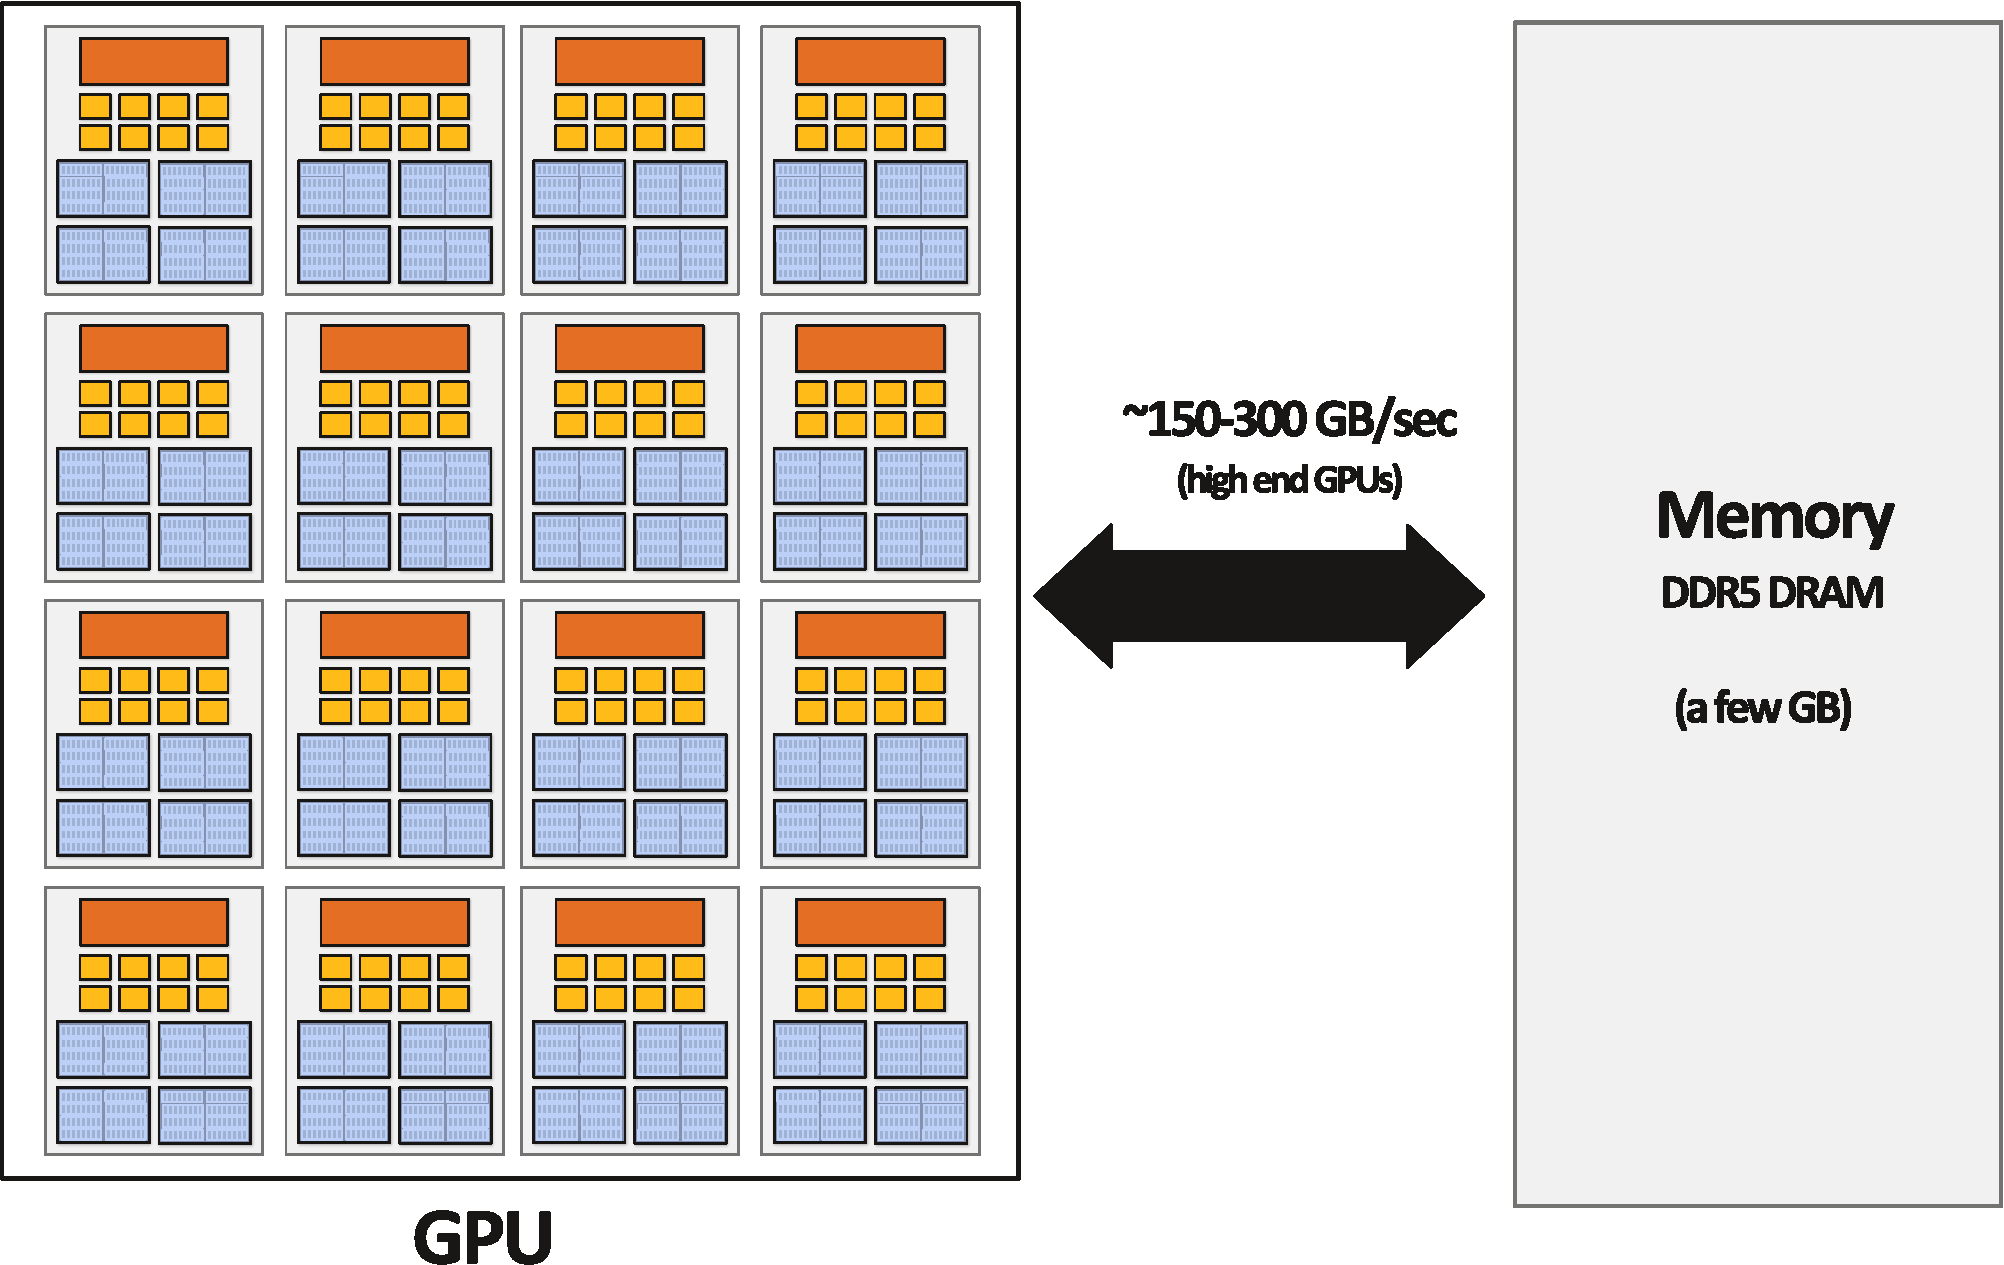
\includegraphics[width=.9\textwidth]{img/gpu-architecture-into-1.pdf}
\end{figure}

\begin{itemize}
    \item \textbf{GPU Structure} (left). The GPU is made up of a \textbf{grid of} smaller blocks, each representing a \textbf{core}. All the blocks form a \textbf{multi-core structure} that allows the GPU to handle many tasks simultaneously.
    
    Within a \textbf{single core}, the GPU uses \textbf{SIMD} (Single Instruction, Multiple Data) \textbf{execution}. This means that many execution units within a core can simultaneously execute the same instruction on different pieces of data. This results in highly efficient execution of parallel tasks such as rendering graphics or running simulations.

    In addition, \textbf{each core supports multi-threaded execution}, which allows multiple threads to be processed simultaneously. This further enhances the GPU's ability to perform multiple tasks simultaneously.


    \item \textbf{Memory Connection} (right). The GPU is connected to DDR5 DRAM, a type of dynamic random access memory. Fast memory is essential to handle the large amounts of data that GPUs process. The more powerful the DRAM, the faster the data transfer.
\end{itemize}
Initially, GPUs were designed with a specific purpose: to render graphics quickly and efficiently. However, their role has expanded significantly over the years.

\highspace
\definition{General-Purpose computing on Graphics Processing Units (GPGPU)} was originally designed to \textbf{render graphics}, but GPUs have evolved to perform a wide range of computations beyond traditional graphics tasks. GPGPU takes advantage of the parallel processing capabilities of GPUs to perform computations typically handled by the CPU.